\documentclass[11pt]{article}
% Figures: \graphicspath, the three ways of sizing an \includegraphics,
% floats with captions and labels, a wrapped figure, and an image captioned
% outside a float. Every file named here is read from disk and embedded in
% the imported document as media, so it travels with the document into
% Markdown, HTML, ODT and DOCX.
\usepackage{graphicx}
\usepackage{wrapfig}
\usepackage{caption}
\graphicspath{{../images/}{../appicon/}}
\title{Figures and Images}
\author{The UltraCanvas Team}
\date{September 2026}
\begin{document}
\maketitle

\begin{abstract}
The document reader resolves every image path against the document's own
directory --- through \texttt{\textbackslash graphicspath} when one is
declared --- loads the file, and stores it in \texttt{document.media}. What
it cannot find it keeps as a placeholder and reports as a diagnostic, so a
broken path is visible rather than silent.
\end{abstract}

\section{Paths}
\texttt{\textbackslash graphicspath\{\{../images/\}\{../appicon/\}\}} lists
the directories to try, in order, for a file given without one.
Figure~\ref{fig:logo} names \texttt{UltraCanvas-logo.png} and is found in
the first of them.

\begin{figure}[h]
  \centering
  
\includegraphics[width=0.45\textwidth]{UltraCanvas-logo.png}
  \caption{A width in fractions of the text width}\label{fig:logo}
\end{figure}

\section{Sizing}
Three spellings of a size are understood, and all of them arrive as points
in the image block:

\begin{itemize}
  \item \texttt{width=0.45\textbackslash textwidth} --- a fraction of the
        article text width, as in Figure~\ref{fig:logo};
  \item \texttt{width=90pt} --- an explicit length, as in
        Figure~\ref{fig:dice};
  \item \texttt{scale=0.4} --- a factor applied to the natural size, as in
        Figure~\ref{fig:texter}.
\end{itemize}

\begin{figure}[h]
  \centering
  \includegraphics[width=90pt]{dice.jpg}
  \caption{An explicit width in points}\label{fig:dice}
\end{figure}

\begin{figure}[h]
  \centering
  
\includegraphics[scale=0.4]{Texter.png}
  \caption{A scale factor, resolved from the second graphics path}\label{fig:texter}
\end{figure}

\section{A figure beside the text}
A \texttt{wrapfigure} is a float like any other as far as the model is
concerned: the text it was meant to flow around simply follows it, because
a rich document has no page to place it on.

\begin{wrapfigure}{r}{0.3\textwidth}
  \centering
  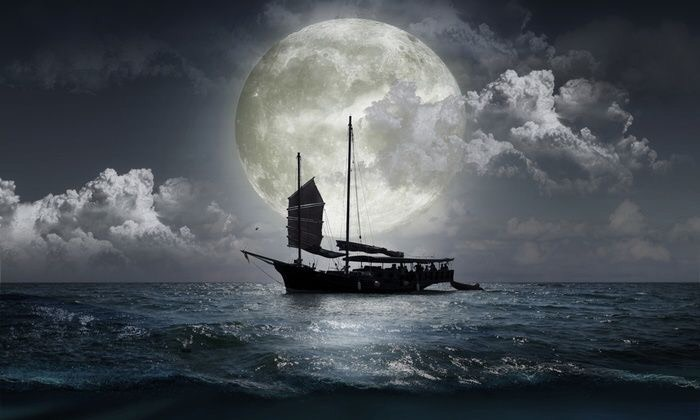
\includegraphics[width=0.25\textwidth]{ship.jpg}
  \caption{Wrapped in the source, stacked in the model}\label{fig:ship}
\end{wrapfigure}

Figure~\ref{fig:ship} keeps its number and its caption; only the placement
is dropped. The same is true of the placement options
(\texttt{[h]}, \texttt{[tbp]}, \texttt{[H]}) on the floats above --- they
say where a typesetter should put the float, and nothing renders them.

\section{An image without a float}
An \texttt{\textbackslash includegraphics} in ordinary text becomes an
image block on its own, and \texttt{\textbackslash captionof\{figure\}}
gives it a number from the figure counter:

\begin{center}
  
\includegraphics[width=0.3\textwidth]{transparent_overlay.png}
\end{center}
\captionof{figure}{A PNG with an alpha channel, captioned outside a float}\label{fig:alpha}

Figure~\ref{fig:alpha} is a PNG with transparency; the image is stored
exactly as it was read, so whatever the renderer makes of the alpha channel
is what the document shows.
\end{document}
